\documentclass[10pt,conference,compsocconf]{IEEEtran}

% After registering, submit here:
% https://cmt3.research.microsoft.com/CILETHZ2016/Submission/Index

%\usepackage{times}
%\usepackage{balance}
\usepackage{url}
\usepackage{graphicx}	% For figure environment

\usepackage{amsmath,amssymb,graphicx}

\usepackage{algorithm}          % Algorithm boxes
\usepackage{algpseudocode}      % Pseudo-code for algorithms
\usepackage{booktabs}			% Pretty tables
\usepackage{color}              % Purdy colors
\usepackage{fontspec}           % Process the diacritics correctly.
\usepackage{listings}           % Code listings.
\usepackage{multirow,tabularx}
\usepackage{tablefootnote}



\begin{document}
\title{CNNs and LSTMs for Sentiment Analysis: A Comparison}

\author{
  Andrei~Bârsan (15-926-777), Bernhard~Kratzwald (15-926-934), Nikolaos~Kolitsas (15-926-405)\\
  Group: Free the Variables!\\
  Department of Computer Science, ETH Zurich, Switzerland
}

\maketitle

\begin{abstract}
	Sentiment analysis has become a very popular machine learning task, as
    more and more companies want to automatically and in real time learn
    what the public thinks about them and their products.
    This paper assess the performance of two state of the art deep learning
    architectures, namely a convolutional and a recurrent neural network,
    comparing their performance against several baselines.
    We show that these architectures significantly outperform classical
    machine learning models, and propose several ways of extending them
    further.
    We also describe a simple but effective preprocessing technique designed
    to leverage word embeddings to their full potential.
\end{abstract}

\section{Introduction}
\label{sec:introduction}

The automatic assessment of sentiment in messages, reviews, and comments
is of great importance for any company with an online presence.

Various machine learning tools have been developed over the past decade with
the goal of automatically classifying whether a piece of text, such as a
restaurant or movie review, carries with it a positive or a negative meaning.
This classification can be either binary (positive or negative), or 
finer-grained. This paper covers the former case.

With this goal in mind, we compare two modern deep learning
models:
a \textbf{convolutional neural network} and
a \textbf{recurrent neural network}. These two
architectures are compared against each other (sections~\ref{sec:cnn} 
and~\ref{sec:rnn}), as well as against several 
traditional machine learning baselines using simple linear models
(section~\ref{sec:baselines}).

While both deep architectures perform substantially better than the traditional
machine learning models, their performance peaks
when used together in a simple binary ensemble, which we describe in
section~\ref{sec:ensemble}.

We also investigate and compare several preprocessing techniques, and assess
the impact of different types of word embeddings~\cite{mikolov2013efficient}.


\section{Models and Methods}
\label{sec:models}

\subsection{Preprocessing}
\label{sec:preprocessing}

The twitter messages that we have to classify are informal text and often contain a lot of spelling mistakes, grammar errors, and non-existent words. In order to improve our classifier's prediction and alleviate these problems, we used an elaborate preprocessing stage.
The misspelled words normally appear in very low frequency (usually only once or twice) and the original preprocessing done by the provided code skeleton just discards all this information.
With our transformations, we try to recover as much information as possible.

\subsubsection{Text substitution}
First of all, by running a Python script, we go through all the tweets and substitute words that contain both characters and numbers with the tag $<$alphanum$>$ (alpha-numberic words) and numbers with the tag $<$num$>$.
For example, ``belkin soho f1ds102l vga and usb 2 port in'' is converted to 
``belkin soho $<$alphanum$>$ vga and usb $<$num$>$ port'', and
``for the next 3 weeks will consist of 7:30- 9:30 up the yard 10:00- 1:00 theatre train''
is converted to 
``for the next $<$num$>$ weeks will consist of $<$num$>$:$<$num$>$- $<$num$>$:$<$num$>$ up the yard $<$num$>$:$<$num$>$- $<$num$>$:$<$num$>$ theatre train''.
Next, all the different hours (7:30, 9:30, 10:00 etc) are treated as the same word $<$num$>$:$<$num$>$, all the different measures (15cm, 28cm, 145cm etc) are converted to the same word $<$num$>$cm, all the different product models are converted to $<$alphanum$>$ etc. This way, we drastically reduce the number of rare words that we encounter in our vocabulary without discarding useful information. 

\subsubsection{Spelling correction}
Tweets contain many misspelled words. The usual solution for spelling correction is to  compare the word with a correct vocabulary (a set of correct words)\footnotemark{} and find appropriate matches with edit distance one or two. However, in our case, a more elaborate solution is needed, since it is very common to encounter on purpose mistakes that have higher edit distance and need special treatment for recovery (e.g. words like
``a-d-o-r-a-b-l-e'', or ``aaaddooooraabblee'').
\footnotetext{We use Google's word2vec pre-trained model due to its richness, having been trained on a corpus of 100 billion tokens.}

For each word, we apply many different techniques, each one returning a set of possible corrections. We then create a union set of all the possible corrections and select the one with the highest probability (most common word).
Some techniques applied are the following:

\begin{itemize}
\item If the word is long enough (above 5 characters) find corrections with $ED \leq 2$ 
(e.g.\ ``morninqq'' $\to$ ``morning''); returns set $S_1$.
\item Delete duplicate letters (``aaaddooooraabblee'' $\to$ ``adorable''); returns set $S_2$.
\item Remove `-' or replace it with whitespace:
(``a-d-o-r-a-b-l-e'' $\to$ ``adorable'', ``labda-calculus'' $\to$ ``labda calculus'');
returns set $S_3$.
\item Split it in two words (``workinghard'' $\to$ ``working hard''), returns set $S_4$.
\end{itemize}

The final correction is the most common word among the union $S_1 \cup S_2 \cup S_3 \cup S_4$. 
\subsubsection{Hashtag manipulation}
Hashtags are usually very informative and help us understand the sentiment of the messages. However, sometimes, instead of using popular, well-known hashtags, users just make their own random concatenation of words.
Our solution does the following to differentiate between these two cases: if the frequency of this hashtag is below a specific threshold\footnote{In most experiments, this is 10 occurrences.}, it is split into simple words (e.g. \#feellikecrying $\to$ feel like crying, \#notgoodnews $\to$ not good news).


\subsection{Word Embeddings}
\label{sec:embeddings}

As embeddings we used 300-dimensional pre-trained google word2vec vectors
whenever available and random initializations otherwise.
We also tried using locally trained word2vec embeddings, as well as a mixture
of pre-trained and locally trained embeddings, both performing worse than the first approach.
Using pre-trained embeddings was a required part of our pre-processing
algorithm, which used them as a pre-existing vocabulary for establishing
whether a particular word existed.

We also experimented with using pre-trained and locally-trained GloVe embeddings~\cite{pennington2014glove},
but they performed worse than word2vec.


\subsection{Baselines}
\label{sec:baselines}

We evaluated our results against two baselines computed using traditional
machine learning models. 

For both these baselines we employed a linear support vector machine (SVM),
whose input features were computed in two different ways. We chose this
classifier because SVMs are a powerful, robust and well-understood technique in classification. 
This approach works fast even for big amounts of data. The optimal regularization
term was determined by 3-fold cross-validation. 

For computing the feature vectors we used two classes of approaches: the former
relies on word embeddings, while the latter employs simple tf--idf term weighting
in a sparse bag-of-words representation.

\subsubsection{Support Vector Machine and Word Embeddings}
For the first baseline, we trained word2vec embeddings on our corpus. For every
tweet, we then averaged its word embeddings, and concatenated them, resulting
in two different vector embeddings for tweets.

Both resulting models were far from accurate (63-67\% accuracy), as can be seen in
section~\ref{sec:results}.


\subsubsection{Support Vector Machine and tf--idf}
The second baseline computes the tf--idf representation of every tweet.

The tf--idf representation of a word in a tweet consists of the product
between the frequency of that term in the tweet and the log of its inverse
document frequency.
%The document frequency of a term is the number of documents in which it appears.
Terms which appear in more than 50\% of the tweets are discarded,
since they provide little discriminatory information.

A tweet is represented in tf--idf format as a
vector populated with the tf--idf score of every word in that tweet. Every
index of the vector corresponds to a unique word ID. Since the corpus is
large (440k+ unique useful words), but an individual tweet is quite short (less 
than 140 characters), these representations are very sparse.

We trained a simple linear SVM classifier on these sparse vectors and achieved
an accuracy of about 80\% (see section~\ref{sec:results}). While this pipeline
did outperform the previous baseline while remaining quite fast to train
(trainable in a few minutes on a laptop CPU), it was still vastly outperformed by
the deeper models showcased in sections~\ref{sec:cnn} and~\ref{sec:rnn}.


\subsection{Convolutional Neural Networks}
\label{sec:cnn}
Convolutional neural networks (CNNs) are used in various tasks such as image and video recognition and Natural Language Processing. They yield state of the art results in text classification~\cite{kim2014convolutional} in general, as well as classification of tweets~\cite{dos2014deep,severyn2015twitter} in specific.

\subsubsection{Input layer} 
CNNs, which have their origin in image classification, require every input to be of the same dimensionality. A tweet is--in analogy to an image--represented as a $N \times D$ matrix, where each row represents a D-dimensional word embedding. The number of rows (words) $N$ is fixed and shorter tweets are filled with a padding word \texttt{<\/PAD>}, while longer tweets are cut off.

We used pre-trained word embeddings as default word representations, as illustrated
in section~\ref{sec:embeddings}. The embeddings are also trained by the neural net.

\subsubsection{Convolutional layer} 
The convolutional layer consists of multiple sliding window functions which are then 
shifted over the input matrix. In contrast to image recognition, each convolution
covers the entire width of the matrix (the entire embedding of a word is covered) but only a specified number of rows (words). The convolutions are then shifted down producing one output for every position in the input matrix. For instance, a convolution of size three
covers three words in the input matrix at once.
Assuming every tweet consists of 30 words, we can shift the convolution down 27 times yielding 28 outputs. We used 384 convolutions in total covering three, four or five words at a time. The final output of the convolution layer is passed to a ReLU activation function.

\subsubsection{Max-pooling and soft-max}
Each of the 384 convolutions produce multiple outputs when being shifted over the input matrix. The next CNN layer pools the maximum of every convolution's output. For instance,
out of the 28 outputs produced by the convolution described above, we keep the
biggest number and discard all 27 others. Applying this to our CNN leaves us with 384-dimensional (number of convolutions) vector. This vector is then used as input for the final soft-max layer generating normalized probability scores for the class assignments. 

\subsubsection{Training and regularization}
The network was trained by stochastic optimization with respect to the cross-entropy-loss. We used the Adam optimizer~\cite{kingmaB14} which is known to work well in practice. We split the input in 90\% training set and 10\% development set.
The training cross-entropy-loss as well as the training classification accuracy were evaluated and logged at every training step. The CNN's performance is then evaluated on the development data after every 1000 training steps. We stopped training after 70k training steps which corresponds to approximately eight epochs (runs through the entire corpus).

To avoid the problem of overfitting we used a dropout layer for convolutions.
The dropout layer disables a neuron during training with a given probability (0.5 in our implementation). Therefore at every training step we used in expectation only half the neurons in our network. This is a very simple and powerful method preventing the NN
from overfitting. 

\subsubsection{Extensions}
We tried using two input channels for the embedding layer. One channel of static word embeddings which are not updated during training and one channel using trainable embeddings as described in~\cite{kim2014convolutional}. The second channel slowed down the training a lot, and wasn't able to significantly outperform the CNN using only one trainable input channel. Therefore, we did not include it for the final model. 


\subsection{Recurrent Neural Networks}
\label{sec:rnn}

In recent years, recurrent neural networks have started showing
a great deal of promise in the field of 
machine translation \cite{sutskever2014sequence}, speech recognition
\cite{graves2013speech}, and sentiment analysis \cite{zhao2016online}. 

Recurrent neural networks are a class of neural networks which contain
inter-unit connections forming a directed graph. Unlike traditional
neural nets, where each component of a data point is fed into the network
simultaneously, recurrent nets are fed input in a sequential fashion.
Their internal state functions
as memory, and they can be used for processing sequential input of varying length,
such as text, handwritten letters, or spoken words.

A common issue with recurrent neural network is their unreliability
when handling long-term dependencies. This occurs due to the need for
propagating error messages over very long distances during backpropagation,
which leads to either exploding or vanishing gradients. This is 
problematic in the field of text processing, where complex sentences can have
very intricate long-term dependencies which dictate their meaning.

The Long Short-Term Memory (LSTM) RNN architecture~\cite{hochreiter1997lstm}
seeks to alleviate these problems by introducing an explicit memory
component into the neural network architectures. These advanced cells can
learn a better way of propagating error messages without gradients shrinking to zero.
Clipping large gradient values is a simple yet effective solution to the second
problem of exploding gradients.

In the past years, LSTM
models have been shown to outperform nearly all traditional RNN architectures
in sequence-based learning tasks, such as
speech recognition~\cite{graves2013speech},
language modeling~\cite{sundermeyer2012lstm},
and sentiment analysis~\cite{zhao2016online}.

For these reasons, we decided to also experiment with an LSTM net.
We started by employing a simple network consisting of an embedding layer,
one layer with 128 LSTM units, and the final softmax. As in our CNN
architectures, the embeddings themselves were also trainable.

While this initial experiment did not outperform our original convolutional
net, it came very close to it in terms of accuracy, as can be seen in
table~\ref{table:accuracy}.
By making the network deeper, with two layers, of 300 and 256 hidden
units respectively, we were able to outperform our CNN on the development
set quite substantially, coming very close to 90\% accuracy.

Interestingly enough, this model did not outperform our CNN on the Kaggle
test data, until it was integrated into a simple ensemble with the
CNN itself.

Additionally, this architecture was considerably slower to train than
the convolutional net, with an epoch taking roughly 4 times longer (2 hours
vs.\ 30 minutes for the convolutional net). Deeper nets were experimented
with, but were prohibitively expensive to train, even on an AWS GPU machine.

For regularizing the LSTM, the training pipeline uses dropout
on non-recurrent connections, as
described in \cite{zaremba2014recurrent},
as well as early stopping whenever
the development set loss starts increasing significantly.

%We also experimented with a 5-layer LSTM with 512 units in each layer,
%and while this model proved very promising, it was also very slow to
%train, remaining underfit even after 36 hours on an AWS GPU.


\subsection{A Simple Ensemble}
\label{sec:ensemble}

While our computational resources did not permit the training of more complex
models, such as a joint LSTM-CNN, we did, however, experiment with simpler
probability averaging for pre-trained model prediction.

This simple approach led us to our best test score by combining our best-performing
CNN and LSTM predictions. The intuition behind this technique's success is
the fact that the two models are very different. This means that, intuitively,
they are able to capture different semantics of the input sentences. And wherever
one single predictor is unsure, in many cases the other one is much more
confident and averaging the probabilities leads to the correct answer.


\section{Results}
\label{sec:results}

\begin{table} \centering
\begin{tabular}[c]{ l c c c }
	\toprule
	\multirow{2}{*}{\textbf{Model}} & \multicolumn{3}{c}{\textbf{Accuracy}} \\
	 & \textbf{Train} & \textbf{Dev} & \textbf{Test} \\
    \midrule
    SVM + Emb. Average & 0.631 & 0.634 & n/a\tablefootnote{\label{note:tbl}Not submitted to Kaggle because of the low development set performance.} \\
    SVM + Emb. Concat & 0.692 & 0.677  & n/a\tablefootnote{See footnote~\ref{note:tbl}.} \\
    SVM + tf--idf & 0.801 & 0.820 & 0.799 \\
    \midrule
    % All are using the second stage of preprocessing.
    CNN & 0.9102 & 0.8734 & 0.8738	 \\
    LSTM (1 layer) & 0.8796 & 0.8732 & 0.8594 \\
    LSTM (2 layer) & \textbf{0.9375} & \textbf{0.8855} & 0.8676 \\
    % We probably shouldn't add this since it's severely underfit, even after 12 epochs.
    % LSTM (5 layer) & 0.9009 & 0.8822 & 0.868 \\
    CNN + LSTM ensemble & 0.9013 & n/a\tablefootnote{This is because the ensemble uses unweighted probability averaging based on the existing, independently trained neural networks.} & \textbf{0.8742} \\
    \bottomrule
\end{tabular}
\caption{Accuracy comparison of the deep models to the baseline.}
\label{table:accuracy}
\end{table}

We have conducted numerous experiments locally, on ETH's Euler
supercomputing cluster, on AWS, and on Google Compute Engine.
All the final experiments employ the preprocessing
stage described in section~\ref{sec:preprocessing}, as it has been shown that
it speeds up training and improves performance, especially for CNNs.

\begin{figure}[tbp]
  \centering
  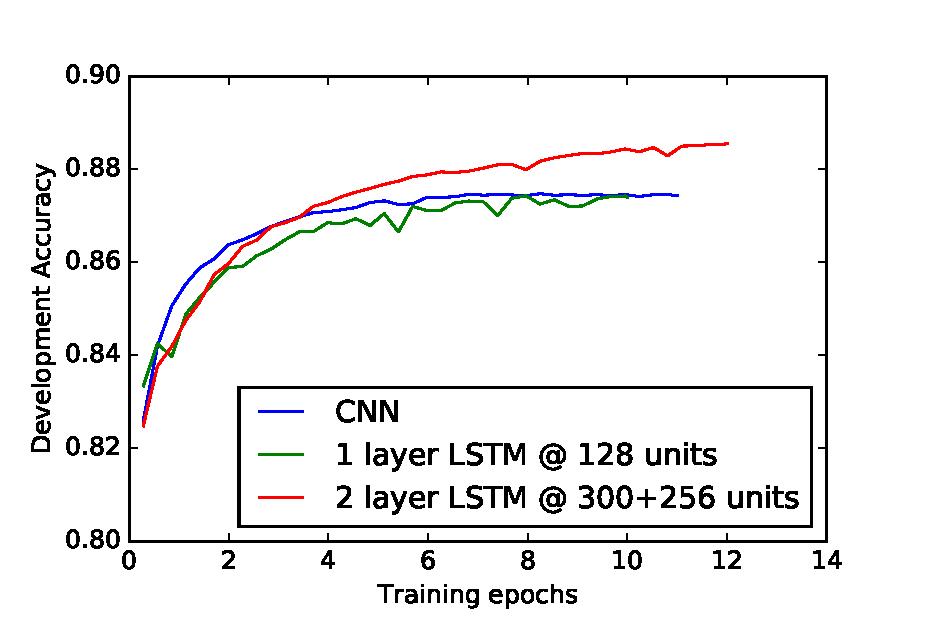
\includegraphics[width=\columnwidth]{cnn_vs_lstm}
  \caption{A comparison of the learning curves for the three best performing architectures. Note that in terms of total training time,
  the LSTMs are considerably slower to train than the CNNs. (Up to 4 times slower.)}
  \label{fig:cnn-vs-lstm}
\end{figure}

Table~\ref{table:accuracy} showcases the main results of our experiments. The model
was trained on 90\% of the 2.5M tweets in the dataset. The remaining 10\% were used
as a development set to ensure no overfitting occurred. The test set is represented
by the 5000 tweets used to compute the (preliminary) Kaggle leaderboard.

Figure~\ref{fig:cnn-vs-lstm} show a comparison of the accuracies of the
three main architectures, as a function of the number of training epochs.
As stated previously, the best-performing individual model is the 2 layer LSTM.
Nevertheless, the overall best test set (Kaggle) results are obtained
by means of a simple averaging ensemble of a CNN and an LSTM.


\section{Discussion}
\label{sec:discussion}

The general deep learning performance trends showcased in the literature have been observed
in our experiments as well.
Convolutional nets are very robust and lead to very good accuracy, while still
being relatively cheap to train.
LSTMs are much more expensive to train, and don't outperform the
convolutional nets until they have at least two layers consisting of 300 and 256 units,
respectively.
Finally, using even a naive ``ensemble'' in the form of probability averaging
pushes the accuracy even further.

Preprocessing has also been shown to help in earlier stages by allowing
the network to e.g.\ start off with better embedding vectors, and to
find more connections between misspelled words. Deeper architectures benefit
somewhat less from the preprocessing, but the difference is still not
negligible.


\section{Summary}
\label{sec:summary}

This paper compared the use of CNNs and LSTMs in the field of binary sentiment
analysis. The final results show that individually, deep LSTMs outperform CNNs,
and that individual models are themselves outperformed by simple ensembles.

Data preprocessing is also important, and can improve training speed especially
in the earlier epochs.

There are still many architectures with could improve text classification
performance. Bidirectional LSTMs have been shown to further enhance 
classification accuracy \cite{zhao2016online}. Accuracy and training speed
could also be improved by employing
\textit{sequential network construction}, as highlighted in \cite{hochreiter1997lstm,fahlman1991recurrent},
whereby an LSTM starts being trained as single-layer, and new layers
are progressively added whenever the error rate stops decreasing.
Ensemble methods and hybrid architectures, such as convolutions and max-pooling
before the LSTM layer are yet another possible path.

\bibliographystyle{IEEEtran}
\bibliography{cil-report}
\end{document}
